\end{multicols}
\section{Results}
In our optimization of the model we iterated over the hyperparemeters in the order: No. of layers, learning rate, debth of layers and kernel size. For each hyperparameter we adjusted the value and allowed the multi-task model to train for 10 epochs and then evaluate accuracy of both the Q8 secondary structure prediction as well as the relative and absolute solvent accessibiliy on both the validation and test set.\\
In choosing which values to continue with for the final model we only considered results on the validation set, and attempted to balance accuracy with model size and trainability.\\
Once we had found what configurations performed the best on the respective parameters, we trained both our single- and multi-task models with these parameters for 20 epochs and compared the results.

\subsection{Hyperparameters}
\subsubsection{No. of layers}
Variying the number of layers in the model greatly affects the size of the model and thus also the time taken to train it. Further, adding more layers increases the risk of overfitting (factcheck lige det...).\\
In our tests we evaluated from two to five hidden layers. Note, that the output layer is not counted in this number.

% Please add the following required packages to your document preamble:
% \usepackage[normalem]{ulem}
% \useunder{\uline}{\ul}{}
\begin{table}[h]
\centering
\begin{tabular}{lcccccc}
\multicolumn{7}{c}{\textbf{No. of layers}} \\
\multicolumn{7}{c}{\textit{Layer debth = 80, kernel size = 11, learning rate = 0.00025, batch size = 4}} \\ \hline
\multicolumn{1}{l|}{} & \multicolumn{3}{c|}{{\ul Validation set}} & \multicolumn{3}{c}{{\ul Test set}} \\
\multicolumn{1}{c|}{Layers} & Q8 & \begin{tabular}[c]{@{}c@{}}Relative\\ solvent\\ accessibility\end{tabular} & \multicolumn{1}{c|}{\begin{tabular}[c]{@{}c@{}}Absolute\\ solvent\\ accessibility\end{tabular}} & Q8 & \begin{tabular}[c]{@{}c@{}}Relative\\ solvent\\ accessibility\end{tabular} & \begin{tabular}[c]{@{}c@{}}Absolute\\ solvent\\ accessibility\end{tabular} \\ \hline
\multicolumn{1}{l|}{2} & 69.79\% & 81.94\% & \multicolumn{1}{c|}{80.58\%} & 69.783\% & 82.001\% & 80.413\% \\
\multicolumn{1}{l|}{3} & 70.08\% & 82.69\% & \multicolumn{1}{c|}{81.10\%} & 70.447\% & 82.259\% & 80.701\% \\
\multicolumn{1}{l|}{4} & 70.11\% & 82.90\% & \multicolumn{1}{c|}{81.18\%} & 70.143\% & 82.291\% & 80.528\% \\
\multicolumn{1}{l|}{5} & 69.48\% & 82.73\% & \multicolumn{1}{c|}{81.13\%} & 69.343\% & 82.158\% & 80.365\% \\
\multicolumn{1}{l|}{16} & 68.15\% & 82.15\% & \multicolumn{1}{c|}{80.42\%} & 68.459\% & 81.595\% & 79.924\% \\
\multicolumn{1}{l|}{32} & 66.94\% & 81.61\% & \multicolumn{1}{c|}{79.85\%} & 67.279\% & 81.196\% & 79.483\% \\
\multicolumn{1}{l|}{64} & 65.10\% & 80.97\% & \multicolumn{1}{c|}{79.25\%} & 65.100\% & 80.644\% & 78.899\%
\end{tabular}
\end{table}
\noindent We made the dicision after this test to continue with 3 hidden layers, as we did not feel that the gained accuracy by advancing to 4 matched the increased cost of training the network.


\subsubsection{Learning rate}
Having a bad learning rate puts the model in risk of several things. A learning rate too small will possibly trap the model in a local minimum, whereas a learning rate too big will risk not being able to hit global maxima, but constantly shifting around them. Further, a lower learning rate means more time needed to train, while a larger learning rate might in the worst case actually miss a global maximum.\\
Below are the results of our tests of learning rate.
% Please add the following required packages to your document preamble:
% \usepackage[normalem]{ulem}
% \useunder{\uline}{\ul}{}
\begin{table}[h]
\centering
\begin{tabular}{lcccccc}
\multicolumn{7}{c}{\textbf{Learning rate}} \\
\multicolumn{7}{c}{\textit{Layer debth = 80, kernel size = 11, 3 hidden layers, batch size = 4}} \\ \hline
\multicolumn{1}{l|}{} & \multicolumn{3}{c|}{{\ul Validation set}} & \multicolumn{3}{c}{{\ul Test set}} \\
\multicolumn{1}{c|}{\begin{tabular}[c]{@{}c@{}}Learning\\ rate\end{tabular}} & Q8 & \begin{tabular}[c]{@{}c@{}}Relative\\ solvent\\ accessibility\end{tabular} & \multicolumn{1}{c|}{\begin{tabular}[c]{@{}c@{}}Absolute\\ solvent\\ accessibility\end{tabular}} & Q8 & \begin{tabular}[c]{@{}c@{}}Relative\\ solvent\\ accessibility\end{tabular} & \begin{tabular}[c]{@{}c@{}}Absolute\\ solvent\\ accessibility\end{tabular} \\ \hline
\multicolumn{1}{l|}{0.00005} & 66.85\% & 81.61\% & \multicolumn{1}{c|}{79.89\%} & 66.958\% & 81.052\% & 79.490\% \\
\multicolumn{1}{l|}{0.0001} & 68.71\% & 82.18\% & \multicolumn{1}{c|}{80.42\%} & 68.983\% & 81.737\% & 80.042\% \\
\multicolumn{1}{l|}{0.00025} & 70.38\% & 82.78\% & \multicolumn{1}{c|}{81.23\%} & 70.386\% & 82.077\% & 80.576\% \\
\multicolumn{1}{l|}{0.0005} & 70.83\% & 82.86\% & \multicolumn{1}{c|}{81.13\%} & 70.624\% & 82.136\% & 80.437\% \\
\multicolumn{1}{l|}{0.001} & 70.66\% & 82.75\% & \multicolumn{1}{c|}{80.92\%} & 70.287\% & 82.040\% & 80.426\% \\
\multicolumn{1}{l|}{0.0025} & 69.12\% & 81.67\% & \multicolumn{1}{c|}{79.59\%} & 68.590\% & 81.294\% & 79.806\%
\end{tabular}
\end{table}
Not only did the non-optimal learning rates not perform as well as 0.0005, but they also trained significantly slower, as seen on the graph below.
\begin{figure}[h]
  \centering
  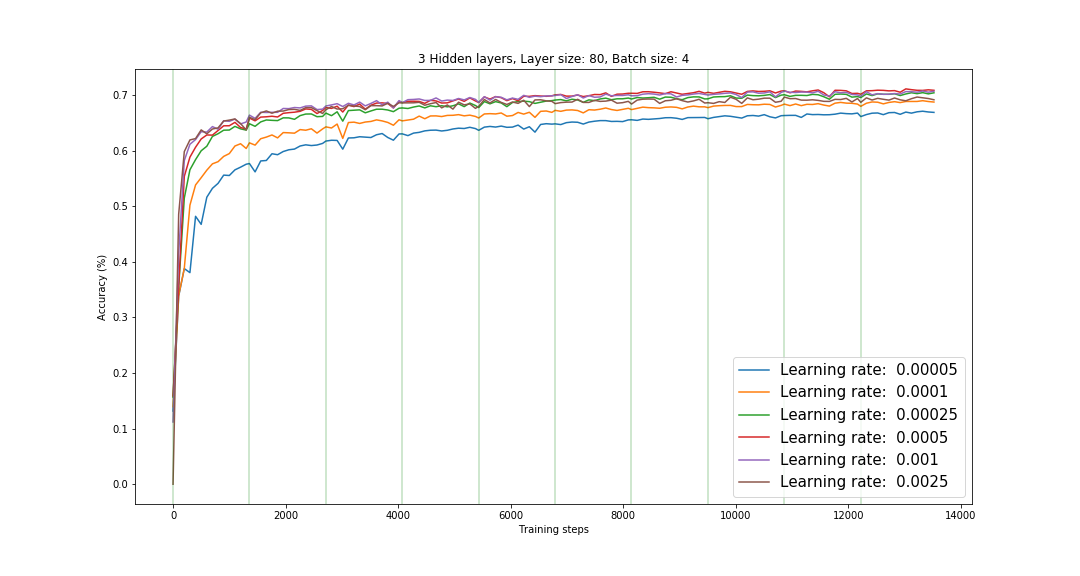
\includegraphics[width=\linewidth]{../graphs/new/learning_rate}
  \caption{Accuracy on the validation with varying learning rate. The green lines represent epochs.}
\end{figure}
For the remainder of the tests we used a learning rate of 0.0005.

\subsubsection{Depth of layers}
As with the number of layers, the depth affects both model potential complex predictive performance and model weight and size. We started from the depth of 100 as also used by Xi et al. and found that no increase in performance was acheived by adding more depth, however some gains were made by shallowing down the layers a bit.

\begin{table}[h]
\centering
\begin{tabular}{lcccccc}
\multicolumn{7}{c}{\textbf{Layer depth}} \\
\multicolumn{7}{c}{\textit{Learning rate = 0.0005, kernel size = 11, 3 hidden layers, batch size = 4}} \\ \hline
\multicolumn{1}{l|}{} & \multicolumn{3}{c|}{{\ul Validation set}} & \multicolumn{3}{c}{{\ul Test set}} \\
\multicolumn{1}{c|}{Depth} & Q8 & \begin{tabular}[c]{@{}c@{}}Relative\\ solvent\\ accessibility\end{tabular} & \multicolumn{1}{c|}{\begin{tabular}[c]{@{}c@{}}Absolute\\ solvent\\ accessibility\end{tabular}} & Q8 & \begin{tabular}[c]{@{}c@{}}Relative\\ solvent\\ accessibility\end{tabular} & \begin{tabular}[c]{@{}c@{}}Absolute\\ solvent\\ accessibility\end{tabular} \\ \hline
\multicolumn{1}{l|}{50} & 70.14\% & 81.94\% & \multicolumn{1}{c|}{81.07\%} & 70.436\% & 82.280\% & 80.395\% \\
\multicolumn{1}{l|}{60} & 70.77\% & 82.68\% & \multicolumn{1}{c|}{81.17\%} & 70.407\% & 81.931\% & 80.295\% \\
\multicolumn{1}{l|}{70} & 70.03\% & 82.97\% & \multicolumn{1}{c|}{81.20\%} & 70.931\% & 82.392\% & 80.723\% \\
\multicolumn{1}{l|}{80} & 70.86\% & 82.78\% & \multicolumn{1}{c|}{81.14\%} & 70.881\% & 82.228\% & 80.535\% \\
\multicolumn{1}{l|}{90} & 71.19\% & 83.09\% & \multicolumn{1}{c|}{81.37\%} & 70.973\% & 82.472\% & 80.734\% \\
\multicolumn{1}{l|}{100} & 70.95\% & 82.05\% & \multicolumn{1}{c|}{80.31\%} & 71.007\% & 82.704\% & 80.602\%
\end{tabular}
\end{table}
\noindent As is seen in the table a depth of 90 filters proved most accurate on our tests. Below is shown a graph of three of the values, illustrating how a depth of 90 performed better than the two other continuously throughout training. Refer to the appendix for at graph containing all the tested  depths.
\begin{figure}[h]
  \centering
  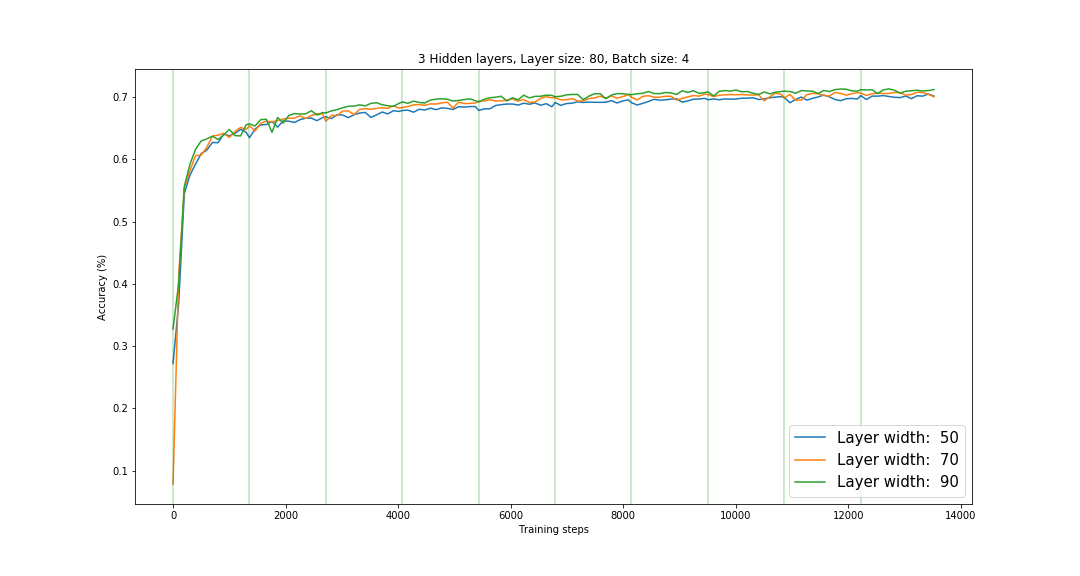
\includegraphics[width=\linewidth]{../graphs/new/layer_width_1}
  \caption{Accuracy on the validation set with varying layer depth.}
\end{figure}
\subsubsection{Kernel size}
Fortæl om kernel sizes og om hvordan vi først prøvede én størrelse på dem alle og siden at variere størrelsen (lav evt. en reference til nogen af dem der har trænet på MNIST og deres kernel sizes), lav en tabel og to grafer.

In the article by Xi et al, a kernel size of 11 was chosen on the basis that the average length 


\begin{multicols}{2}

\subsection{Final predictive capabilities}
Forklar hvordan vi fandt frem til vores hyperparametre på multi-task modellen og så anvendte de samme på single-task. Skriv noget tekst om hvordan vi på test-sættet nåede op på so-and-so meget præcision på hhv. den ene og anden model og hhv. strukturer og solvent egenskaber, samt sammeligning af resultatet på test- og valideringssæt.


\subsection{Comparison}
Forklar hvordan de to modeller ender med næsten samme præcision, omend multi-task modellen tager langt længere tid om at komme derop. De convergerer (jeg tror ordet er 'predictive ceiling') begge omkring de 68.5\%, men for single allerede omkring 10 epoker medens multi skal bruge 25 epoker.
